\documentclass[preview]{standalone}
\usepackage{tikz}
\usepackage{pgfplots}
\usepgfplotslibrary{smithchart}
\usepgfplotslibrary{polar}
\pgfplotsset{compat=1.11}

\begin{document}
    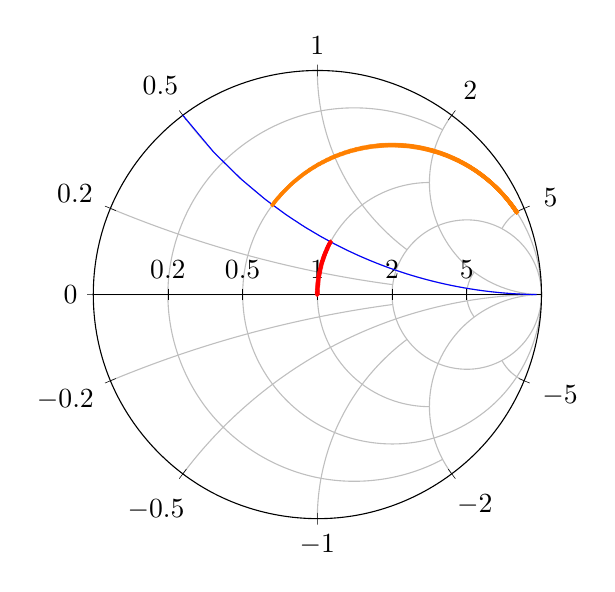
\begin{tikzpicture}
        \begin{smithchart}
            
    %     \path[draw=red, thick] (0pt,0pt) circle (1.5cm);
        % \path[draw=blue] (0.2,0.5) circle (0.75cm);
        %% Admittance plot
        \addplot[domain=0:90,samples=600, color=blue] {.5};

        % \addplot[domain=0:90,,samples=600, color=green] {-2};
        % \addplot[domain=0:90, samples=600, color=red] {5};

        % \addplot[data cs=polarrad,domain=0:2*pi] (\x,1);
        % \addplot[data cs=polarrad,domain=0:2*pi] (\x,1);
    %     \path[draw=blue,fill=blue] (0.2,0.5) circle (0.05cm);
    %     % \addplot  coordinates  {(0.5,0.2)  (1,0.8)  (2,2)};
    %     \addplot[mark=none,line width=1]
    %    coordinates{
    %        (1, 0) (1, 0.1) (1,0.2) (1,0.3) (1,0.4) (1,0.5) (1,0.5) (1, 0.6) (1, 0.7) (1, 0.8) (1, 0.9) (1, 1)
    %    };
    %    \foreach \a in {0,.1,...,1}{
    %     \addplot[mark=none,line width=1]
    %     coordinates{
    %         (1, \a)
    %     };

    % \addplot[samples=10,domain=0:1] {(x)^2};
        \foreach \x in {.5, .51,...,5}
        {\edef\temp{\noexpand\addplot+[mark=*,
        mark options={solid},color={orange},mark size=.2,line width=1] coordinates { (.5,\x) };}\temp}


        \foreach \x in {0, .01,...,.5}
        {\edef\temp{\noexpand\addplot+[mark=*,
        mark options={solid},color={red},mark size=.2,line width=1] coordinates { (1,\x) };}\temp}

        

        % {\edef\temp{\noexpand\addplot+[mark=*,
        % mark options={solid},color={red},mark size=.2,line width=1] coordinates { (.5,sin(2*\p)*cos(2*\p)) };}\temp}

    % \addplot coordinates {\foreach \x in {.1,...,.9}  (\x,0) (\x,1)};

    % \foreach \y in {0,.01,.02,...,1}
    % {\edef\temp{\noexpand\addplot+[mark=o,
    % ,color={blue},] coordinates { (\y,-0.2) };}\temp}
    

    % \foreach \y in {0,.25,...,50}
    % {{\addplot+[mark=*,
    % mark options={solid},color={green},] coordinates { (\y,-2) };}}
    
        \end{smithchart}
        % \begin{polaraxis}

                % equivalent to (x,{sin(..)cos(..)}), i.e.
                % the expression is the RADIUS
                % \end{polaraxis}
    \end{tikzpicture}
\end{document}